\subsection{Kennisgewing onderdeel}

Die kennisgewing onderdeel is verantwoordelik vir die hantering van alle
kennisgewings in die stelsel, insluitend push-kennisgewings, stelsel
kennisgewings, en toestel registrasie. Dit laat beide gebruikers en
administrateurs toe om kennisgewings te ontvang, te bestuur, en te
konfigureer.

\begin{figure}[H]
    \centering
    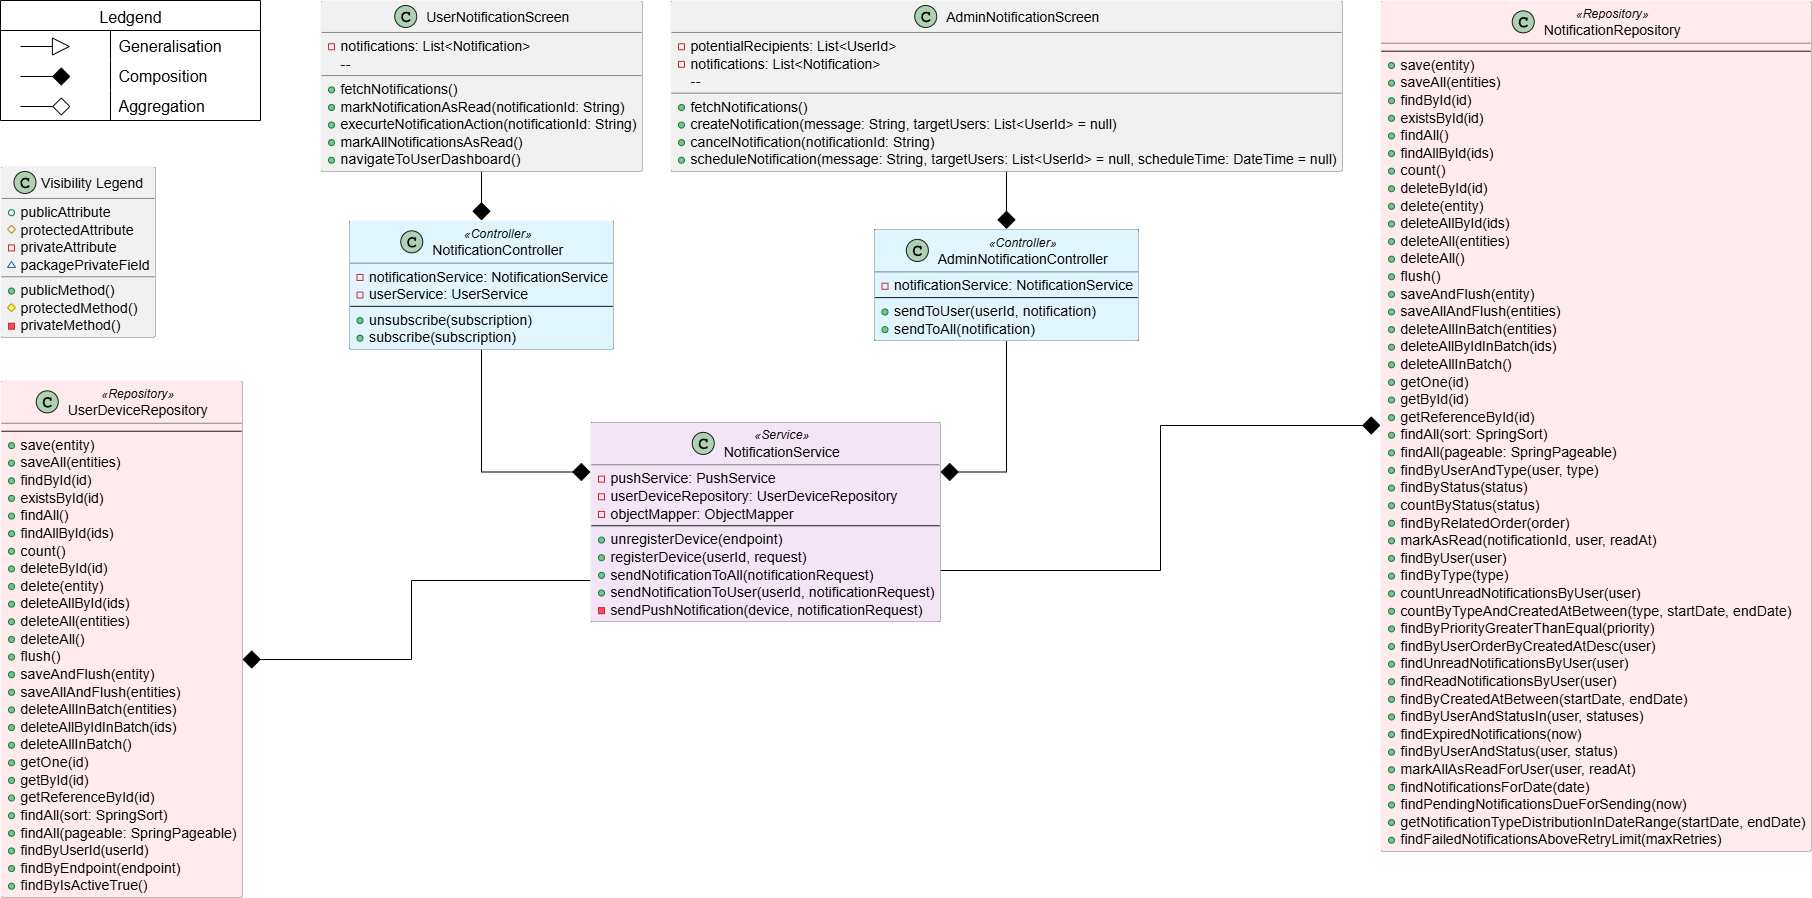
\includegraphics[width=\textwidth]{figures/class_diagrams/notification-subsystem.png}
    \caption{Kennisgewing onderdeel klasdiagram}
    \label{fig:notification_subsystem_class_diagram}
\end{figure}

Hier volg die CRC kaarte vir die belangrikste klasse in hierdie
onderdeel.

\textbf{AdminNotificationScreen} laat administrateurs toe om kennisgewings te skep, te stuur, te skeduleer en afleweringstatus te monitor.
\begin{table}[H]\centering\begin{tabular}{|p{0.4\textwidth}|p{0.4\textwidth}|}
    \hline
    \multicolumn{2}{|c|}{\textbf{AdminNotificationScreen}} \\
    \hline
    \textbf{Verantwoordelikhede} & \textbf{Medewerkers} \\
    \hline
    Skep en stuur kennisgewings na gebruikers \newline
    Skeduleer kennisgewings vir later aflewering \newline
    Bestuur stelselwye kennisgewings \newline
    Kyk kennisgewing aflewering status
    &
    AdminNotificationController \\
    \hline
\end{tabular}
\caption{CRC vir AdminNotificationScreen}
\label{tab:crc_admin_notification_screen}
\end{table}

\textbf{AdminNotificationController} hanteer administratiewe kennisgewingversoeke, verwerk skepping en skedulering, en verskaf statistieke.
\begin{table}[H]\centering\begin{tabular}{|p{0.4\textwidth}|p{0.4\textwidth}|}
    \hline
    \multicolumn{2}{|c|}{\textbf{AdminNotificationController}} \\
    \hline
    \textbf{Verantwoordelikhede} & \textbf{Medewerkers} \\
    \hline
    Hanteer administratiewe kennisgewing versoeke \newline
    Verwerk kennisgewing skepping \newline
    Bestuur kennisgewing skedulering \newline
    Verskaf kennisgewing statistieke
    &
    NotificationService \\
    \hline
\end{tabular}
\caption{CRC vir AdminNotificationController}
\label{tab:crc_admin_notification_controller}
\end{table}

\textbf{UserNotificationScreen} bied gebruikers die vermoë om kennisgewings te besigtig, as gelees te merk en voorkeure te bestuur.
\begin{table}[H]\centering\begin{tabular}{|p{0.4\textwidth}|p{0.4\textwidth}|}
    \hline
    \multicolumn{2}{|c|}{\textbf{UserNotificationScreen}} \\
    \hline
    \textbf{Verantwoordelikhede} & \textbf{Medewerkers} \\
    \hline
    Wys gebruiker se kennisgewings \newline
    Merk kennisgewings as gelees \newline
    Voer kennisgewing aksies uit \newline
    Bestuur kennisgewing voorkeure
    &
    NotificationController \\
    \hline
\end{tabular}
\caption{CRC vir UserNotificationScreen}
\label{tab:crc_user_notification_screen}
\end{table}

\textbf{NotificationController} hanteer gebruikerskennisgewingversoeke, bestuur toestelregistrasie en verwerk leesstatus.
\begin{table}[H]\centering\begin{tabular}{|p{0.4\textwidth}|p{0.4\textwidth}|}
    \hline
    \multicolumn{2}{|c|}{\textbf{NotificationController}} \\
    \hline
    \textbf{Verantwoordelikhede} & \textbf{Medewerkers} \\
    \hline
    Hanteer gebruiker kennisgewing versoeke \newline
    Bestuur toestel registrasie vir push-kennisgewings \newline
    Verwerk kennisgewing lees status
    &
    NotificationService \\
    \hline
\end{tabular}
\caption{CRC vir NotificationController}
\label{tab:crc_notification_controller}
\end{table}

\textbf{NotificationService} verwerk en stuur kennisgewings, bestuur toestelregistrasie, aflewering, stoor en skedulering.
\begin{table}[H]\centering\begin{tabular}{|p{0.4\textwidth}|p{0.4\textwidth}|}
    \hline
    \multicolumn{2}{|c|}{\textbf{NotificationService}} \\
    \hline
    \textbf{Verantwoordelikhede} & \textbf{Medewerkers} \\
    \hline
    Verwerk en stuur kennisgewings \newline
    Bestuur toestel registrasie \newline
    Hanteer push-kennisgewing aflewering \newline
    Stoor en verkry kennisgewings \newline
    Bestuur kennisgewing skedulering
    &
    NotificationRepository \newline
    UserDeviceRepository \\
    \hline
\end{tabular}
\caption{CRC vir NotificationService}
\label{tab:crc_notification_service}
\end{table}

